% Use the "Template" class with specified options and set page margins
\documentclass[10pt,a4paper]{Template}
\geometry{left=1cm,right=1cm,top=1cm,bottom=1cm} % Set custom page margins

% Import packages for encoding, fonts, math, etc.
\usepackage[utf8]{inputenc}
\usepackage[T1]{fontenc}
\usepackage[default]{lato}
\usepackage{amsmath}
\usepackage{amssymb}
\usepackage{physics}
\usepackage{tikz}
\usepackage{relsize}
\usepackage{scalefnt}

% Beginning of the document
\begin{document}

% Reset page style
\thispagestyle{empty}

% Header of the document
\makeheader[Mathematics]{Linear Algebra Cheat Sheet}

% First column of the page
\begin{minipage}{0.48\textwidth}

\topic[Vector Operations]

\subtopic{Vector Basics}
\vspace{-5mm}
\[ \vu*\rvec = \frac{\rvec}{\norm{\rvec}} \;\; \text{(Unit Vector)}\]
\[ \norm{\rvec} = \sqrt{\rvec^2_1 + \rvec^2_2 + \cdots + \rvec^2_n} \;\; \text{(Norm)} \]
\divider

\subtopic{Dot Product}
\vspace{-5mm}
\[ \rvec \cdot \svec = \rvec_{i} \svec_{i} + \dots + \rvec_{n} \svec_{n} \]
\[ \rvec \cdot \svec = \norm{\rvec} \norm{\svec} \cos{\theta} \]
\begin{itemize}
	\item If $\theta = 90^{\circ}$ then $\rvec \cdot \svec = 0 $
	\item If $\theta = 0^{\circ}$ then $\rvec \cdot \svec = \norm{\rvec} \norm{\svec} $
	\item If $\theta = 180^{\circ}$ then $\rvec \cdot \svec = - \norm{\rvec} \norm{\svec} $
\end{itemize}
\divider

\subtopic{Projections}
\[ \frac{\rvec \cdot \svec}{\norm{\rvec}} \;\; \text{(Scalar Projection of $\svec$ onto $\rvec$)}\]

\[ \frac{\rvec \cdot \svec}{\rvec \cdot \rvec} \rvec = \frac{\rvec \cdot \svec}{\norm{\rvec} \norm{\rvec}} \rvec \;\; \text{(Vector Projection of $\svec$ onto $\rvec$)}\]
\divider

\subtopic{Basis}
\vspace{0.15cm}
A basis is a set of n vectors that:
\begin{itemize}[topsep=2.5pt]
	\item are not linear combinations of each other;
	\item span the space.
\end{itemize}
The space is then n-dimensional. \\

{\small \faLightbulb} \ A vector is independent of one or more vectors if it cannot be represented as a linear combination of them. This means:
\[ \vvec_1 \not = c_1 \vvec_{2} + \dots + c_n \vvec_{n} \]

\vspace{0.5cm}

\topic[Matrices]

\subtopic{Identity}
\[
I
= \begin{bmatrix} 
1 & 0 & \cdots & 0\\ 
0 & 1 & \cdots & 0 \\ 
\vdots & \vdots & \ddots & \vdots \\ 
0 & 0 & \cdots & 1
\end{bmatrix} 
\; \text{(Identity Matrix)}
\]

\vspace{0.30cm}

\divider

\subtopic{Determinant (2x2 Matrix)}
\[ \det \begin{bmatrix}
a & b \\ 
c & d
\end{bmatrix}
= 
a d - b c 
\] 
\begin{itemize}
    \item The determinant indicates how much the transformation can dilate or compress the space.
    \item $\det(I)$ is always equal to 1.
    \item If the vectors that make up a matrix are linearly dependent, the determinant will be equal to zero. 
\end{itemize}
\divider
  
\end{minipage}
\hfill
% Second column of the page
\begin{minipage}{0.48\textwidth}
\vspace{0.66cm}

\subtopic{Inverse (2x2 Matrix)}
\[A^{-1} A = I \;\]
The product between the matrix and its inverse is always the identity matrix.
\[
\begin{bmatrix}
a & b \\ 
c & d
\end{bmatrix}^{-1}
=\frac{1}{a d - b c }
\begin{bmatrix}
d & -b \\ 
-c & a
\end{bmatrix} 
\; \text{(Inverse Calculation)}
\]
{\small \faLightbulb} \ A square matrix is invertible only if its determinant is non-zero. If the determinant is zero, the matrix is called \textbf{singular} and does not have an inverse. \\

There is a method known as "Gauss elimination" that can be used to find the inverse of a matrix. This method involves reducing the original matrix to a "stepped reduced" form by elementary operations on the rows.
\divider

\subtopic{Matrix Multiplication}
Summation convention for multiplying matrices a and b:
\[(AB)_{ij} = \sum_{k} A_{ik} B_{kj}\]

\[
AB
=
\begin{bmatrix}
\sum_{k=1}^{n} A_{1k}B_{k1} & \dots & \sum_{k=1}^{n} A_{2k}B_{kn} \\
\vdots & \ddots & \vdots \\
\sum_{k=1}^{n} A_{mk}B_{k2} & \dots & \sum_{k=1}^{n} A_{mk}B_{kn}
\end{bmatrix}
\]
\divider

\subtopic{Change of Basis}
If we have a transformation matrix $B$ where the columns are the new basis vectors in the original coordinate system:
\[B \rvec = \svec\]
and consequently:
\[B^{-1} \svec = \rvec\]


If a matrix $A$ is \textbf{orthonormal} (all the columns are of unit size and orthogonal to eachother) then:
\[A^T = A^{-1}\]
\divider

\subtopic{Gram-Schmidt Process for Constructing an
Orthonormal Basis}
Start with $n$ linearly independent basis vectors \\ $\vvec =
\{\vvec_1, \vvec_2, \dots, \vvec_n\}$. Then:
\[ \evec_1 = \frac{\vvec_1}{\norm{\vvec_1}}\]
\[ \uvec_2 = \vvec_2 - (\vvec_2 \cdot \evec_1) \evec_1 \;\; \text{so} \;\; \evec_2 = \frac{\uvec_2}{\norm{\uvec_2}}\]
and so on for $\uvec_3$ being the remnant part of $\vvec_3$ not
composed of the preceding $\evec$-vectors, etc$\dots$

\divider

\end{minipage}

\null\newpage

% Reset page style
\thispagestyle{empty}

\begin{minipage}{0.48\textwidth}

\topic[\relscale{0.886} Transformations \& Reflections]
Here is the approach for transforming vectors into a higher space using reflections and linear transformations:
\begin{enumerate}[topsep=2.5pt]
    \item \textbf{Transformation into the Reflection Plane Base ($E^{-1}$)}: the vector of interest is transformed into the basis of the plane of reflection.
    \item \textbf{Application of the Reflection or Desired Transformation ($T_E$)}: the desired reflection or other transformation in the plane of the object is performed.
    \item \textbf{Return to Original Base ($E$)}: the transformed vector is returned to the original base.
\end{enumerate}
So the transformed vector ($\rvec'$) is obtained through the following formula: $\rvec' = E \cdot T_E \cdot E^{-1} \rvec$. \\

This approach allows manipulating vectors in a higher space by combining reflections and linear transformations, offering a powerful and systematic method for examining and manipulating geometric objects in this context.

\vspace{0.5cm}

\topic[Eigenstuff]
\subtopic{Eigenvalues and Eigenvectors}
The \textbf{eigenvectors} (or characteristic vectors) of a matrix are nonzero vectors that, when multiplied by that matrix, result only scaled by a value known as the \textbf{eigenvalue} (or characteristic value). \\

There is a fundamental relationship that is of great importance, namely, $A x=\lambda x$, where $A$ is a square matrix of dimension $n \times n$, $x$ is a nonzero vector, and $\lambda$ is a scalar (the eigenvalue) associated with $x$. This equation can be rewritten as $(A-\lambda I)x=0$, where $I$ is the identity matrix of dimension $n \times n$. \\

To find the eigenvalues $\lambda$ of the matrix $A$ we can solve $\det(A-\lambda I)=0$. This characteristic polynomial is zero, and the solutions of this polynomial are the eigenvalues of the matrix $A$. \\

Once the eigenvalues have been found, we can calculate the eigenvectors associated with each eigenvalue by solving the equation $(A-\lambda I)x=0$. The eigenvectors are the nonzero vectors $x$ that satisfy this equation. \\

To summarize, eigenvalues and eigenvectors are important because they provide crucial information about the behavior of the linear transformation represented by the matrix $A$.

\divider

\subtopic{Eigenvalue Decomposition}
Given a matrix $T$, we would like to perform repeated transformations of a vector v. Unfortunately, if we perform $T^n v$, the computation can be computationally quite onerous. What we do is to perform eigenvalue decomposition to simplify the repeated transformations. \\

1. \textbf{Eigenvector Matrix ($C$)}: Find the eigenvectors associated with $T$ and arrange them as columns in matrix $C$:

\[ C = \begin{bmatrix} v_1 & v_2 & \dots & v_n \end{bmatrix} \]

\end{minipage}
\hfill
% Second column of the page
\begin{minipage}{0.48\textwidth}

\vspace{-7.1675cm}

2. \textbf{Diagonal Eigenvalue Matrix ($D$)}: Organize the eigenvalues of $T$ along the main diagonal of matrix $D$, and zeros elsewhere:

\[ D = \begin{bmatrix} 
\lambda_1 & 0 & \dots & 0 \\
0 & \lambda_2 & \dots & 0 \\
\vdots & \vdots & \ddots & \vdots \\
0 & 0 & \dots & \lambda_n \\
\end{bmatrix} \]

3. \textbf{Inverse of the Eigenvector Matrix ($C^{-1}$)}: Compute the inverse of matrix $C$. \\

Now, the eigenvalue decomposition of matrix $T$ is expressed as:

\[ T = C \cdot D \cdot C^{-1} \]

So, decomposition to eigenvalues allows us to represent a \textbf{matrix as the product of three matrices} and this allows us to simplify operations like raising $T$ to a power $n$, where we can use the decomposition to obtain $T^n$ as:

\[ T^n = C \cdot D^n \cdot C^{-1} \]

Here, $D^n$ is the matrix obtained by raising each eigenvalue of $T$ to the power $n$ while maintaining the diagonal structure. \\

Using this decomposition, we can significantly simplify the calculations associated with $T$ and its powers, making the analysis and application of repeated transformations easier. See the graph below for a better understanding:

\vspace{0.3cm}
\begin{center}
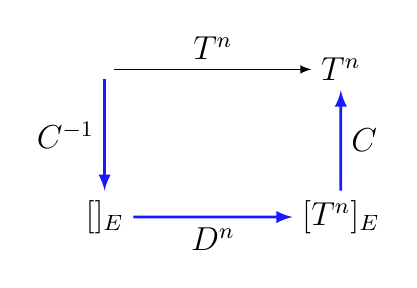
\begin{tikzpicture}[>=latex, scale=1.5]
  % Nodes
  \node (a) at (0,0) {\large$\vvec$};
  \node (b) at (2,0) {\large$T^n \vvec$};
  \node (c) at (0,-1.25) {\large$[\vvec]_E$};
  \node (d) at (2,-1.25) {\large$[T^n \vvec]_E$};
  % Arrows
  \draw[->] (a) -- node[above] {\large$T^n$} (b);
  \draw[->, line width=1pt, Blue!90] (a) -- node[left] {\color{black}\large$C^{-1}$} (c);
  \draw[<-, line width=1pt, Blue!90] (b) -- node[right] {\color{black}\large$C$} (d);
  \draw[->, line width=1pt, Blue!90] (c) -- node[below] {\color{black}\large$D^n$} (d);
\end{tikzpicture}
\end{center}

\divider

\end{minipage}

% End of the document
\end{document}